\documentclass[10pt]{article}
\usepackage{amsmath,graphicx,fullpage,float}
\title{User Space Provenance Tool}
\date{\today}
\author{Thomas Bytheway, Nikilesh Balakrishnan}
\begin{document}
\maketitle
\section{Introduction}
Reproducibility is gaining importance in the scientific community as the quantity of data produced grows and software work-flows become increasingly complex. Over the years numerous attempts have been made in order to capture the computational and data provenance of systems.


\section{Requirements}
The requirements for the first phase of our system the following requirements apply:
\begin{itemize}
\item The system must be capable of capturing provenance in terms of the relation between files and processes.
\item The system must require minimal user intervention and setup.
\item The system must incur a minimal overhead to the users activities.
\item The system must allow the user to query the stored provenance in an approachable fashion.
\end{itemize}

\section{Development Decisions}
\subsection{Classes of Provenance Capture Method}
\begin{itemize}
\item Provenance API
\item Workflow Systems
\item Userland Tracing
\item OS Tracing
\end{itemize}

Provenance APIs and Workflow systems are not especially appealing given our requirements as both techniques require large amounts of user or programmer intervention.

\subsubsection{Userland Tracing}
\paragraph{FUSE}
Good filesystem level tracing, high overheads and requires that the user shadow their filesystem in a subdirectory.
\paragraph{libc interception}
Broad system call capture, low overheads, vulnerable to statically linked libraries and direct system calls.
\paragraph{ptrace}
Full system call interception, high overheads, arcane and abstruse interface.
\paragraph{Binary Rewriting}
Add trampolines to the binary being executed whenever a system call instruction is encountered. Provides full system call interposing capabilities. Difficult to implement correctly. Involves a lot of development time and effort.
\paragraph{Linux audit subsystem}
Powerful but rigidly specified capture capabilities, only a single configuration per machine allowed, system admin orientated. 
\paragraph{SystemTap}
Very powerful system call capture, provides scripting language with embedded C, can have high overheads, requires root permissions and requires Linux debug symbols to be installed.

\subsubsection{OS Tracing}
\begin{description}
\item[kprobes] Flexible kernel debugging and tracing, low overheads, requires root permissions, available only from 2.6.9 kernel and requires kernel to be compiled with CONFIG\_KPROBES enabled.
\item[System call table interception] Very powerful system call capture, requires root permissions, requires modifying page permissions, requires finding address of system call table.
\item[Linux security modules] Powerful capture capabilities, only a single KSM can be loaded (preventing users from also running SELinux), misses any system calls that fail before permissions checks.
\end{description}

\subsection{Database Paradigms}

\subsubsection{RDBMS}
RBDMS are conventionally used to store related records under a specific schema format. However they struggle to represent graph structures efficiently and result in exceedingly complex queries to traverse paths in such a database.

\subsubsection{Graph Databases}
Graph databases can represent our provenance object relationships effectively and allow for powerful querying capabilities. However most graph databases are distributed, proprietary or otherwise suited for much heavier weight systems. The initial phase of the project requires a simpler approach to represent provenance objects and hence graph databases have been ruled out for the first phase.

\subsubsection{Key/Value Stores}
Key/value stores are a quick and easy way to store provenance objects, they do not require a specific schema and provide a simple if less powerful interface for querying. Key/value stores are available for a range of applications from heavy weight distributed systems to single node systems using an embedded database. In phase one of the system we are focusing on a single node application and an embedded key/value store will cater to our requirements.



\section{Assumptions}
\begin{itemize}
\item Targeting linux using the current ABI
\item Targeting x86/x86\_64
\item Assume most programs use libc to make system calls
\item Assume most programs are dynamically linked
\item Assume purelibc intercepts all system calls made via libc
\end{itemize}

\section{Design}

\subsection{Overview}
\begin{figure}
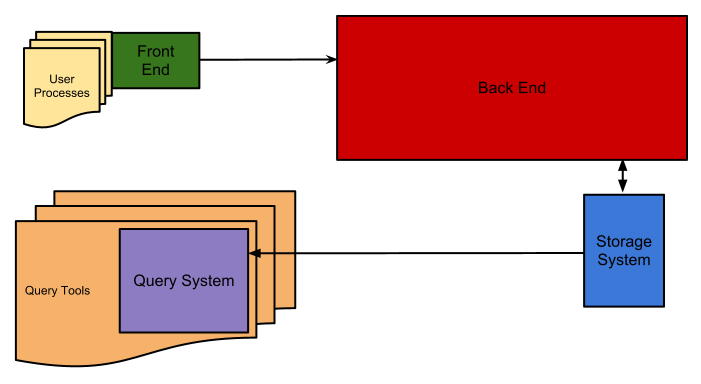
\includegraphics[width=\textwidth]{res/BroadProvDesign.png}
\label{fig:broaddes}
\caption{Broad design of the provenance system.}
\end{figure}
The system will consist of four main parts.
\begin{enumerate}
\item A front end which captures provenance data from the users activities.
\item A back end which processes raw provenance data into related provenance objects.
\item A self contained storage system which persists provenance objects.
\item A query API which will return provenance objects to user tools.
\end{enumerate}
The system will be designed such that it would be possible to run several instances of front end systems simultaneously.

In our initial implementation we are planning to use a libC based system call interception technique in our front end to capture user provenance data transparently and with low overhead. We are planning to use a local key/value store for our initial storage system.


\subsection{Module Level Design}
\begin{figure}
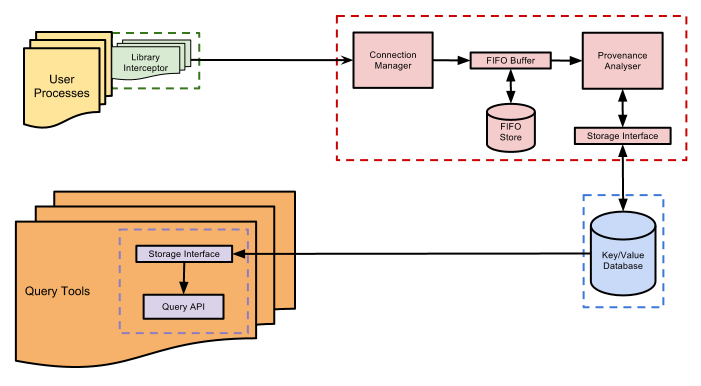
\includegraphics[width=\textwidth]{res/ProvDesign.png}
\label{fig:detdes}
\caption{Detailed design of the provenance system.}
\end{figure}

\subsubsection{Library Interceptor}
The front-end will consist of a shared library implemented in C++, which will be pre-loaded before the user application starts execution. The shared library can be loaded during the start of a shell session and will track all activities that the user performs during that session. The front-end will monitor a subset of libc function calls (mainly I/O) and transmit the data to the back-end via a Unix Domain Socket (UDS). The data will be packaged using Google's Protocol buffers as they provide a convenient and extensible format for messages. Each monitored I/O event will be tagged with a monotonic counter to indicate the actual completion of the I/O event.

\subsubsection{Connection Manager}
The back-end will consist of a thread which can accept UDS connections from the front-end clients. For each connection its corresponding UDS file descriptor will be added to the list of descriptors being monitored for data. The raw libc function data will be persisted to a log file on disk before being input into a priority queue which orders the data received based on the system's monotonic counter.

\subsubsection{Persistent Log file}
The persistent log file will provide us with the capability to analyse and debug the tool during development. It also offers the user the capability to resume a provenance trail in an event of a system or process crash. An index of checkpoint locations within the log file will also be maintained as it can provide an efficient way to rollback and resume our provenance data creation step.

\subsubsection{Provenance Analyser}
The provenance analyser thread will pull out raw provenance data from the priority queue and convert it data into logical provenance objects and relations. If multiple clients send provenance data from the front-end, the back-end may not receive the data in the exact order in which the I/O events occured on the system. This could potentially cause the provenance graph to be generated incorrectly. The priority queue will ensure that the messages are ordered by their monotonic counter values. A window length for processing the messages in the queue will also be enforced.

\subsubsection{Storage Interface}
The storage interface uses a key/value database to store provenance objects. It will present a strict interface to the rest of the system allowing provenance objects to be stored and retrieved and for iteration over ranges of provenance objects. We will be implementing this using an embedded key/value database called levelDB, our justification for such can be found in Section \ref{levelDBJust}. 

\subsubsection{Key/Value Database}
The key/value store will feature four levelDB databases (tables in relational parlance). They are as follows,
1. File and process records identified by unique provenance IDs (provID).
2. I/O information for processes and files identified by I/O IDs (ioID).
3. An index that maps entity names to a list of provIDs.
########
The second database will one acting as the main data store and two acting as indexes to this. The main database will map provenance identifiers (provID) to provenance objects (see section \ref{POF}). Provenance identifiers will be unique monotonically increasing integer identifiers, they will monotonically increase to allow for a strong mapping between time and provenance identifier. The first index will map entity names to a list of all provenance entities that hold that name, ordered by increasing provID. This will allow new entries to simply be appended to the list. The second index will map timestamps to appropriate provIDs, this will be filled by inserting entries at boundaries in timestamp(e.g. every hour or every minute) containing the timestamp and the last used provID. Thus by rounding a time period to the nearest boundaries you can obtain a range of provIDs that describes the time period.

\subsubsection{Query API}
The query API will provide a wide variety of functions for retrieving provenance objects from the storage interface. It will be available initially as an importable module which any query tool can use. The strict definition of it's API has not yet been created as further investigation into the form of provenance queries needs to be made.


\subsection{Interface Specification}
\subsubsection{Unix Domain Socket Messaging Format}
\label{ProvProt}
\begin{table}[H]
\begin{tabular}{|l|l|}
\hline
Field Name & Field Type\\
\hline
Message Type & char\\
Message Length & int\\
\hline
\end{tabular}
\caption{Message Header}
\end{table}

Message type may take one of a series of enumerated values. The logical values are SETUP, SYSCALL and AGGREGATE. SETUP and SYSCALL message headers will be followed by a setup or syscall message as detailed below. AGGREGATE message headers are followed by a series of message header, message pairs. The purpose of aggregate messages is to allow both the front and back end to make bulk writes/reads to the socket to gain greater performance.

\begin{table}[H]
\begin{tabular}{|l|l|}
\hline
Field Name & Field Type\\
\hline
EXE Name Length & int\\
CWD Length & int\\
\hline
\multicolumn{2}{|c|}{String Data}\\
\hline
\end{tabular}
\caption{Setup Message}
\end{table}

\begin{table}[H]
\begin{tabular}{|l|l|}
\hline
Field Name & Field Type\\
\hline
syscall Number & int\\
Arguments & int64*6\\
Return & int64\\
Timestamp & int64\\
String Arguments & char\\
\hline
\multicolumn{2}{|c|}{String Data}\\
\hline
\end{tabular}
\caption{Syscall Message}
\end{table}

The string arguments element is a single byte bitfield that indicates which arguments are strings. String arguments will have the character pointer that would be in the argument slot replaced with a length and the string data appended to the end of the message in argument order.

\subsubsection{Provenance Object Format}
\label{POF}
\inputminted{protobuf}{../prov_db.proto}


\subsection{Tool Choices}

\subsubsection{PureLibc}
\label{PurelibcJust}
Purelibc is a tool implemented in C which performs library interception. We chose not to use Purelibc to implement our front end as while minimises the amount of work needed, it shortcuts the library calls to system calls rather than calling the original library function, thus may not mimic the behaviour of glibc exactly. Purelibc has some drawbacks in that  it has not implemented some secondary system calls, also purelibc is licensed with GPL.

\subsubsection{Protocol Buffers}
\label{ProbufJust}
Implementing the serialisation and deserialisation of objects can be cumbersome and language dependent. Protocol buffers offer an extensible and language independent system for data serialisation. Protocol buffers offer an interface description language that can be compiled into C++, Java or Python using language specific protocol compilers.

\subsubsection{Python}
Python was chosen for the majority of the system because of the wide array of tools that it provides and the rapid development speed that it can bring. It will result in a faster development cycle at the expense of higher overheads, we hope this can be mitigated somewhat by use of c extensions.
\subsubsection{levelDB}
\label{levelDBJust}
The first version of the system will use levelDB in the storage system as it is an embedded ordered key/value store. It supports memory caching and iterating over ranges of keys. It is implemented in c++ but presents bindings for a number of languages including python. The use of levelDB makes the storage of information just an API call rather than relying on IPC methods such as in database connections for SQL.
\subsubsection{Unix domain sockets}
In order to communicate between the front and back end of the system we need to use an IPC mechanism. Unix domain sockets provide an ordered, local and low overhead mechanism for IPC on Unix systems. 



\end{document}
